\documentclass{article}

\usepackage{url}
\usepackage{graphicx,subfig}
\usepackage{float}
\usepackage{fullpage}
\usepackage{amsmath}


\title{Beyond Linearity / Something New / Summary}
\author{Nolan McCafferty}

\usepackage{Sweave}
\begin{document}
\Sconcordance{concordance:project4.tex:project4.Rnw:%
1 12 1 1 0 3 1 1 13 1 1 1 26 11 1 1 10 1 2 7 0 1 2 1 3 1 2 4 1 1 4 1 2 %
7 0 1 2 1 3 1 2 2 1 1 8 1 2 4 1 2 2 3 1 1 12 1 2 6 1 1 26 1 2 22 1 1 11 %
1 2 4 1 1 4 13 0 1 2 2 1 1 7 1 2 7 1 1 4 34 0 1 2 7 1 2 2 6 1}

\maketitle





\section*{Sparse and Smooth Linear Models}

\subsection*{Introduction}

The dataset I am using for this project is a set of NFL play-by-play data from 2009-2017. I have narrowed down the data to the subset of data I want to work with, play-by-play data for the Seattle Seahawks from 2013-2015, in order to conduct inference on the Seahawks from 2009-2017. The observational unit is one play in a football game and there are over 75 columns for each play with several numerical and categorical variables including season, down, yards-to-go, play-type, and many more (that being said there are many columns that would be inappropriate in building a model). The response variable in my analysis is the yards-gained on the play. I have added several more explanatory variables into the anlysis including Firstdown, Time in seconds, quarter, drive, Touchdown, Yards-after-catch, and more. 

\subsection*{Ridge Regression and LASSO}

Using CV we see that the optimal lambda for our RR model is :


\begin{Schunk}
\begin{Sinput}
> hawks.rr.cv$lambda.min
\end{Sinput}
\begin{Soutput}
[1] 0.0433
\end{Soutput}
\end{Schunk}

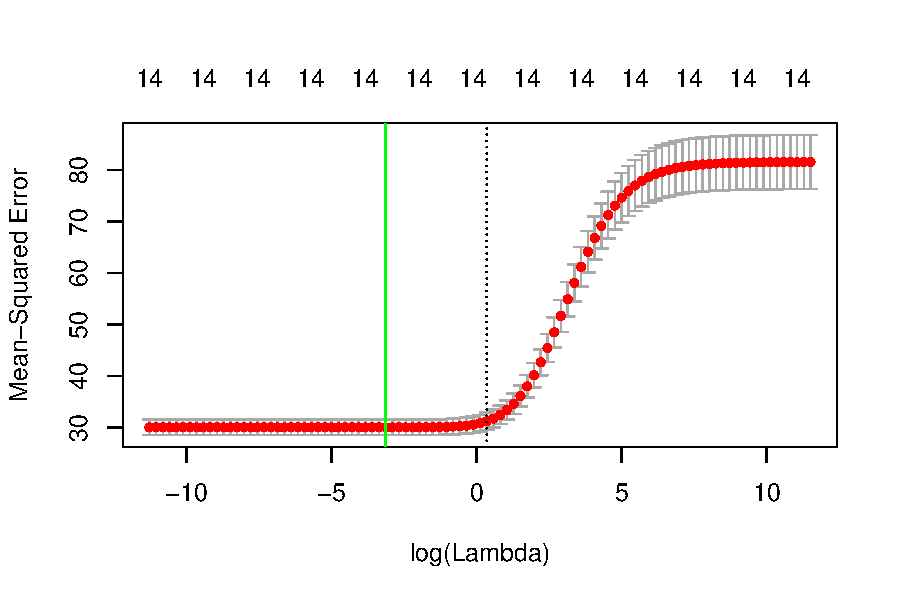
\includegraphics{project4-005}

\newpage

We see that the optimal lambda for our LASSO model is :


\begin{Schunk}
\begin{Sinput}
> hawks.lasso.cv$lambda.min
\end{Sinput}
\begin{Soutput}
[1] 0.0272
\end{Soutput}
\end{Schunk}

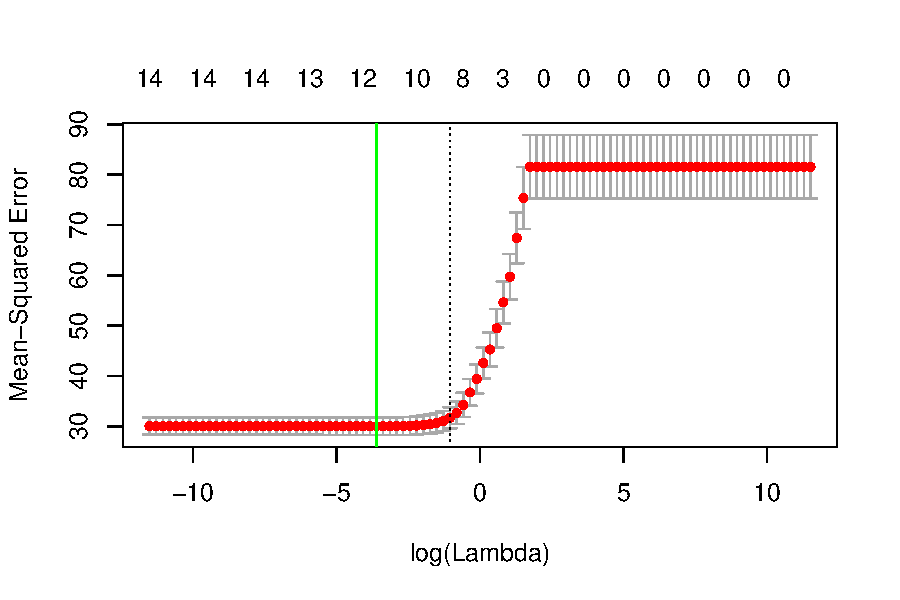
\includegraphics{project4-008}

The plots below show that the Ridge Regression and LASSO coefficients are almost identical. The two large coefficients correspond to the variables Firstdown and Timesecs. Firstdown is a binary variable that shows if the play resulted in a first down or not. It makes sense that this variable would have an impact because if the play results in a firstdown then there must be yards-gained by definition. Timesecs is the amount of seconds remaining in the game, so earlier in the game this value will be large and it decreases as the game goes on. The large coefficient implies that more yards are gained earlier in the game rather than at the end, which makes sense (because teams could be running out the clock or taking a knee at the end). 

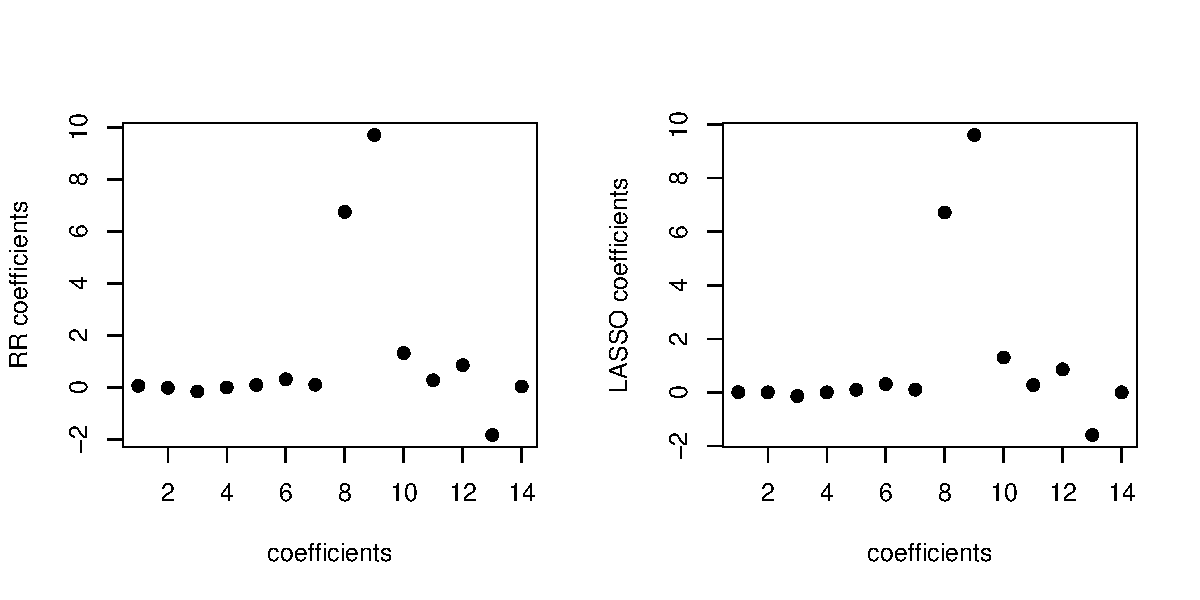
\includegraphics{project4-009}

\newpage

The coefficients for the MLR model (with the added variables) are shown in the plot below. We see that Firstdown again has a high coefficient and Touchdown also has a high coefficient. 

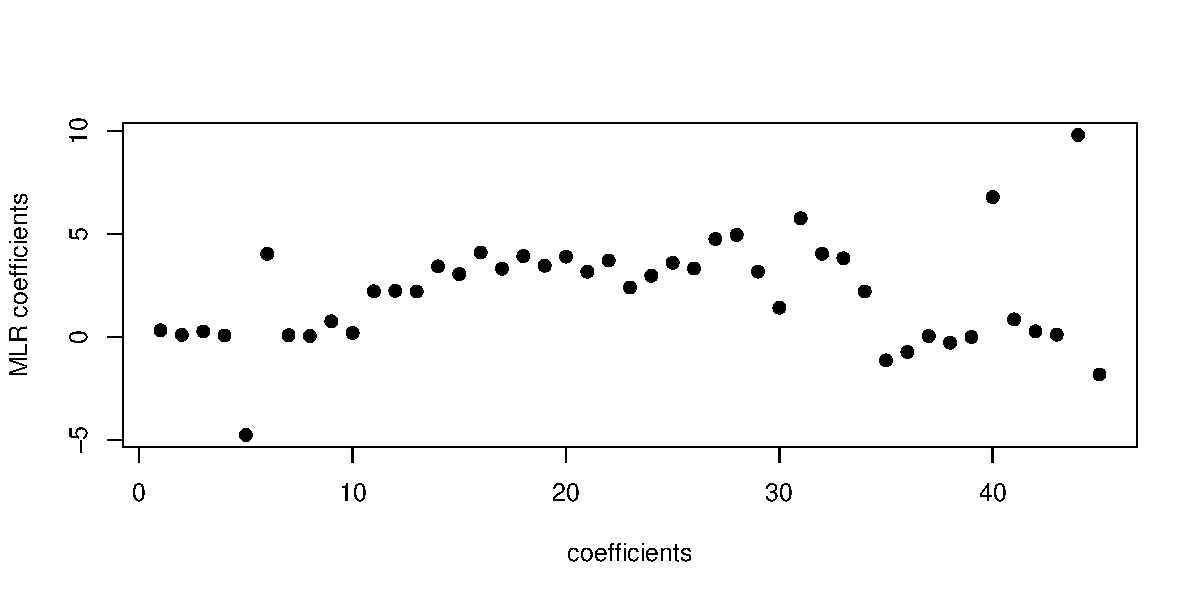
\includegraphics{project4-010}


The plot of the predictions of each model is below. For the predictions I used the data from the 2017 Seahawks Season. As you can see, the RR and LASSO models are almost identical in their predictions. Also, the MLR model consitently predicts slightly below the RR and LASSO models. The predictions generally follow the $y=x$ line (which they should if they predict correctly). 

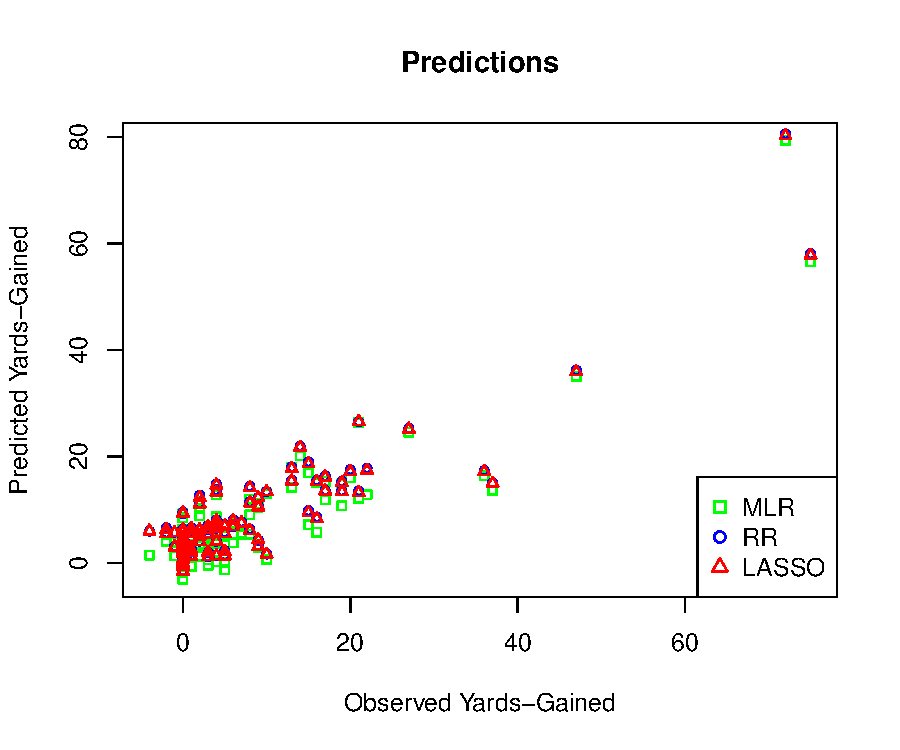
\includegraphics{project4-011}





\subsection*{Regression Splines and Local Regression}

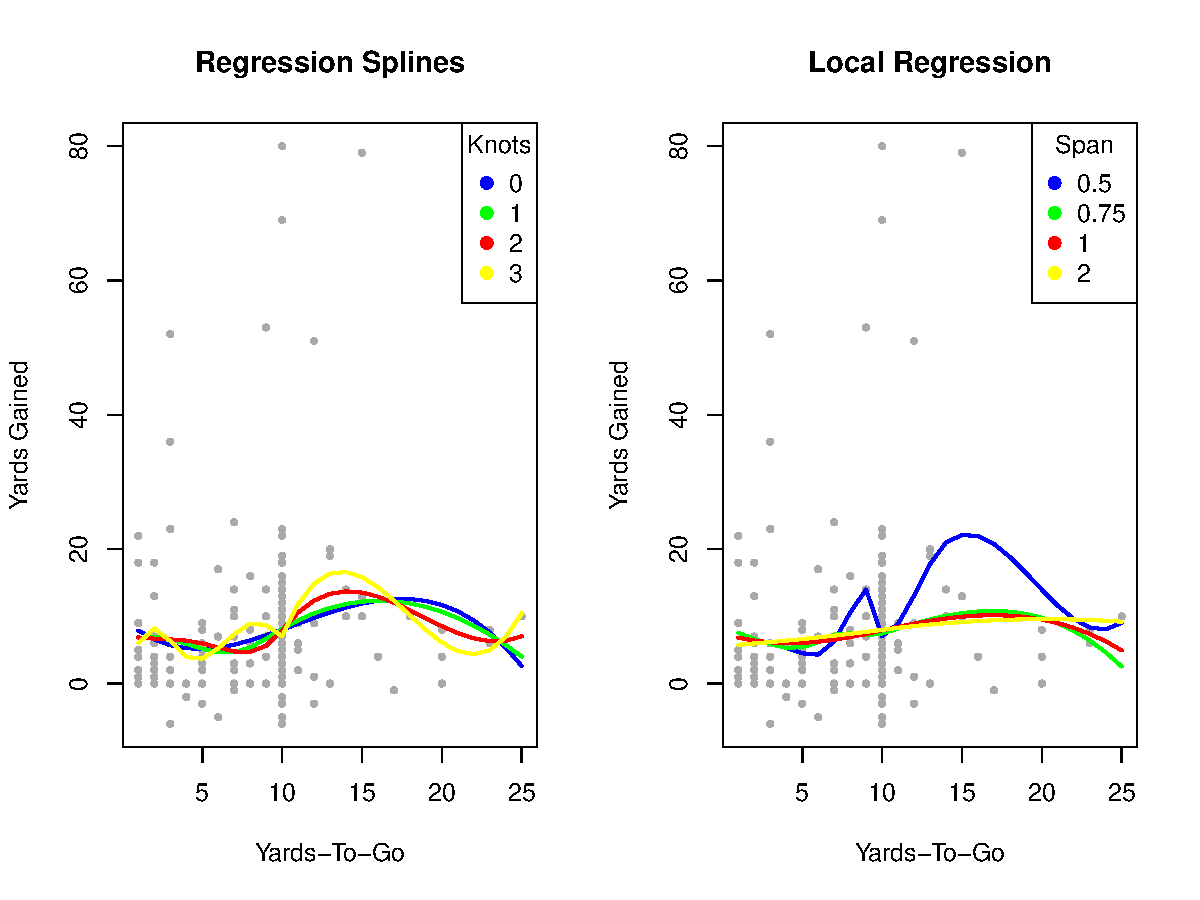
\includegraphics{project4-012}

The plot above on the left shows four regression spline models, all degree 3, each with a different number of knots. As you can see, the models all give similar fits for the data, however it is clear that the models with more knots are overfitting the data. Consistant across all the models is the slow increase in slope until just after 10 yards followed by a steady decrease. On the right above are four local regression models with different spans. Similarly, the models with very small spans are overfitting and the general shape is consistent. 

\section*{Something New}

\subsection*{Local Regression in Higher Dimensions}

For the additional analysis using a concept we have not discussed in class, I will explore Local Regression (kernels) in higher dimensions. I picked this method because it is clear from the initial kernel smoother models that the Yards-To-Go variable in particular does not have a linear relationship with the response (Yards-Gained). Therefore, using kernel smoothing methods could produce a better model than just linear models. Extending Local Regression to higher dimensions is an interesting concept because defining the "neighborhood" of an observation becomes more difficult as well as visualizing the predictions. 

When extening Local Regression to multiple dimensions, it is important to think about what happens to the "neighborhood" of a specific observation. Since there are now two or more dimensions to consider, the number of points in the local neighborhood of an particular point will decline. This presents a problem because we need there to be a fixed number of points in each local regression. The solution comes via altering a parameter, span. This will cause the span to be larger, which means the regression will become less local causing the bias of the estimate to increase. 

The mechanics of Multidimensional Local Regression are very similar to the loess model in one dimension. Weighted Least Squares is used to fit each local regression model and the span is chosen to smooth the data. The difference with multiple explanatory variables is that we must take the product of all the marginal weights to find the neighborhood of each observation:

$$w_{i} = W(\frac{D(x_{i}, x_{0})}{h})$$

where $W$ is the weight function and $D(x_{i}, x_{0})$ is the distance (Euclidean in R) between the particular $x_{0}$ and each $x_{i}$ and $h$ is the window half-width. 

\vspace{5mm}

For our Seahawks data, we will use yards-to-go and yard-line as the explanatory variables in our multidimensional local regression. The plots below show the predictions for several different span values:

\vspace{1cm}

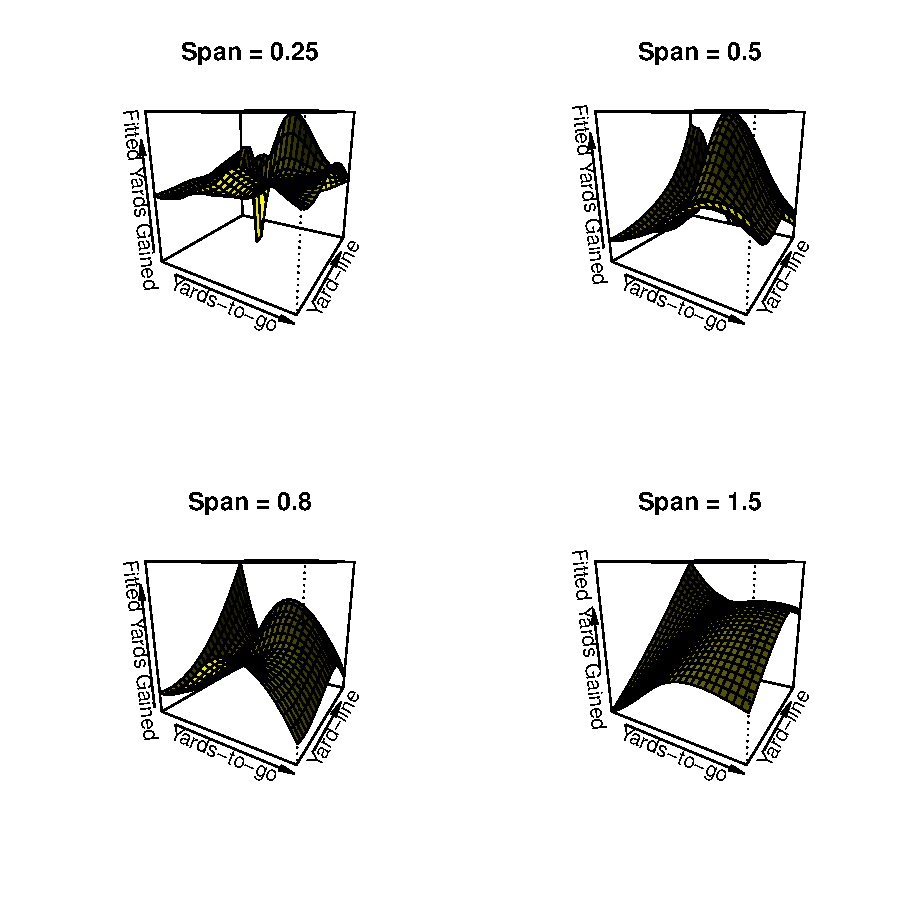
\includegraphics{project4-013}

\newpage

We can see from the plots above that the regression surface is clearly nonlinear. The plot with span = 0.8 seems to not overfit the data while still providing an interesting surface. Next, we conduct an incremental F-test for the terms in the model:

\begin{Schunk}
\begin{Soutput}
Model 1: loess(formula = Yards.Gained ~ ydstogo + yrdline100, data = hawks, span = 0.8)
Model 2: loess(formula = Yards.Gained ~ ydstogo, data = hawks, span = 0.8)

Analysis of Variance:   denominator df 2822

      ENP    RSS F-value  Pr(>F)    
[1,] 10.3 224702                    
[2,]  5.1 228999    7.12 3.4e-08 ***
---
Signif. codes:  0 ‘***’ 0.001 ‘**’ 0.01 ‘*’ 0.05 ‘.’ 0.1 ‘ ’ 1
\end{Soutput}
\end{Schunk}

Using the ANOVA function above, we see that there is a significant difference when yard-line is added to the model (p-value < 1e-07)! Here is our final model (3D is cool):

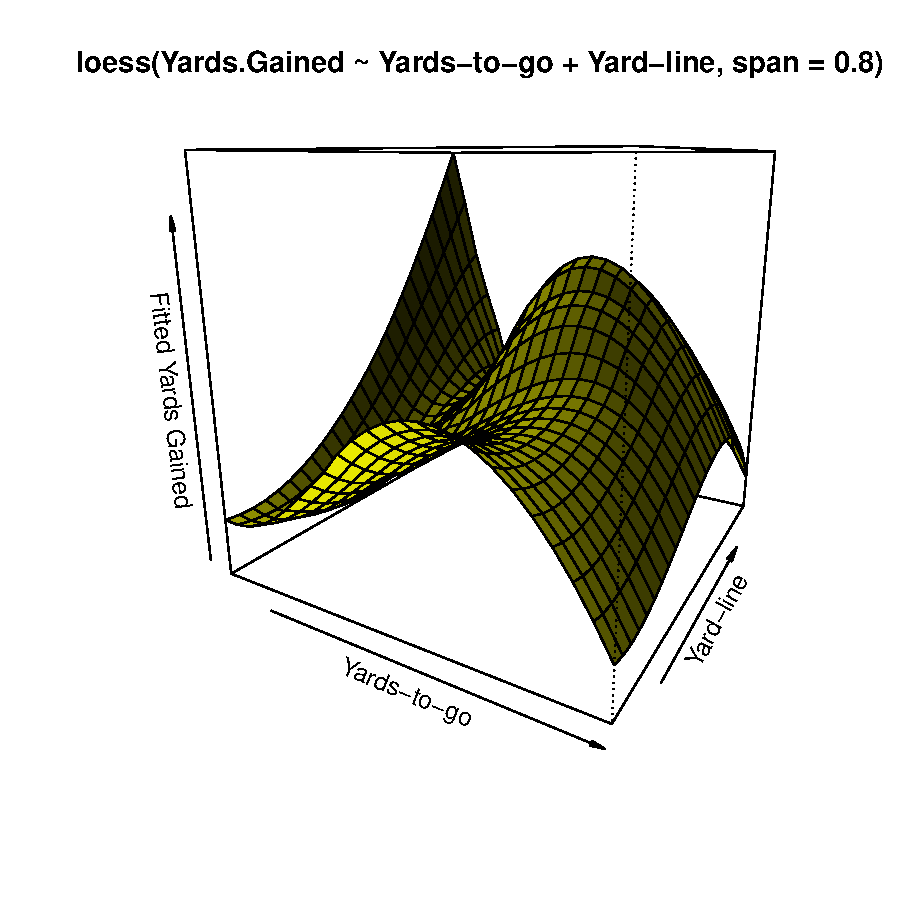
\includegraphics{project4-015}

\newpage

\section*{Summary}

By adding more explanatory variables to the model (especially Firstdown and Touchdown), I was able to improve my model drastically from the last project. The final model is given below:


\begin{Schunk}
\begin{Soutput}
Call:
lm(formula = Yards.Gained ~ ydstogo * PlayType + yrdline100 + 
    down + FirstDown + YardsAfterCatch + AirYards + ydsnet + 
    Touchdown + Fumble, data = hawks)

Residuals:
   Min     1Q Median     3Q    Max 
-24.70  -2.84  -0.33   2.37  55.76 

Coefficients:
                     Estimate Std. Error t value Pr(>|t|)    
(Intercept)         -10.18788    0.58388  -17.45  < 2e-16 ***
ydstogo               0.21613    0.03732    5.79  7.8e-09 ***
PlayTypeRun           2.27860    0.50867    4.48  7.8e-06 ***
yrdline100            0.09179    0.00592   15.52  < 2e-16 ***
down2                 0.34406    0.24060    1.43    0.153    
down3                 0.00940    0.29670    0.03    0.975    
down4                -4.61853    0.99556   -4.64  3.7e-06 ***
FirstDown1            6.94546    0.26162   26.55  < 2e-16 ***
YardsAfterCatch       0.86749    0.02418   35.88  < 2e-16 ***
AirYards              0.28232    0.01431   19.72  < 2e-16 ***
ydsnet                0.10176    0.00611   16.66  < 2e-16 ***
Touchdown1            9.91383    0.54071   18.33  < 2e-16 ***
Fumble1              -1.76288    0.90988   -1.94    0.053 .  
ydstogo:PlayTypeRun   0.21435    0.05061    4.24  2.4e-05 ***
---
Signif. codes:  0 ‘***’ 0.001 ‘**’ 0.01 ‘*’ 0.05 ‘.’ 0.1 ‘ ’ 1

Residual standard error: 5.41 on 2820 degrees of freedom
Multiple R-squared:  0.643,	Adjusted R-squared:  0.641 
F-statistic:  390 on 13 and 2820 DF,  p-value: <2e-16
\end{Soutput}
\end{Schunk}
  
This new model has an Adjusted R-squared of 0.641, compared to the Adjusted R-squared of 0.047 for the previous model gives a increase of 0.594! Suddenly, the model actually seems significant and accurate for the data. Analyzing the coefficients of the model reveals several interesting findings. First, the explanatory variables "down4" and "Fumble1" have negative coefficients, indicating that if it is fourth down, or there is a fumble on the play, the prediction of yards-gained decreases. Another interesting observation is that "down2" and "down3" do not seem to be significant (high p-values) but "down4" has a very small p-value. This tells us that there is little difference between if it is second or third down, but if it fourth down there is a signifiant decrease in expected yards-gained. The variables "Firstdown1" and "Touchdown1" have the largest coefficients, which makes sense because to get a firstdown or touchdown you have to gain yards. I also interacted yards-to-go with play-type for the final predictor. 


\newpage

The residual plot is given below:

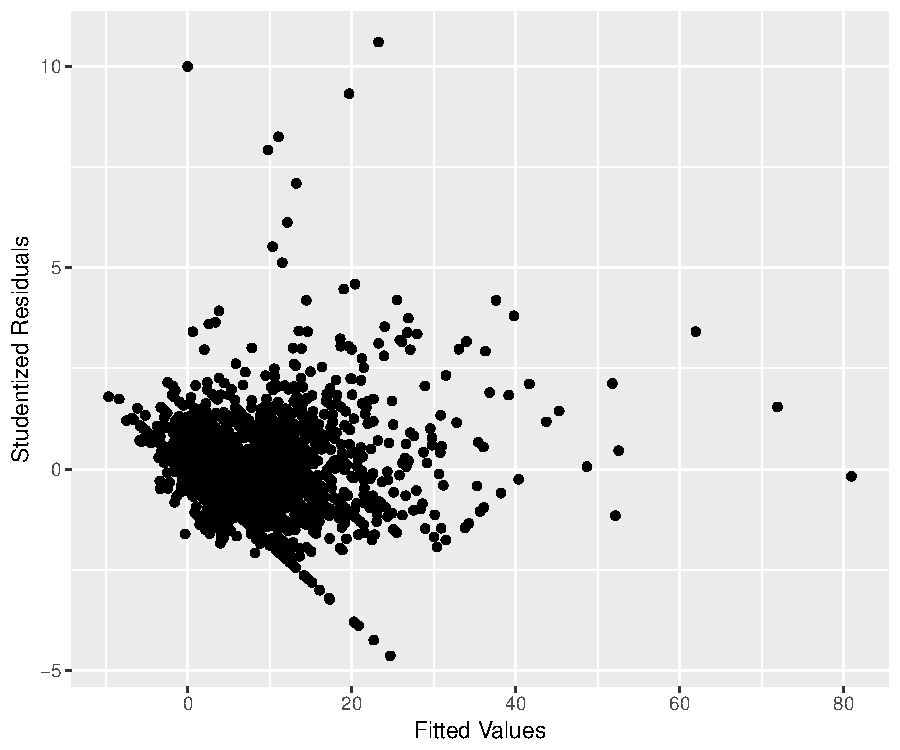
\includegraphics{project4-017}

The addition of these variables completely changed the entire outlook of my project. I was fully prepared to present a narrative of repeated failed anlalysis and a model with little to no value. However, this final model gives actual insight into the data and holds predictive power. I can't give you a realistic situation where you would ever need to predict the yards gained on a specific football play given these explanatory variables, but if that problem ever arises this model could be very useful. The process of repeated modeling using several different techniques opened my eyes to these new variables that turned out to be influential. 

An interesting extension to this project could be building a model like this for different teams throughout the NFL and seeing if the model changes significantly from team to team. An interesting note is that throughout the models I was unable to find any significance from the Season variable. This could be because the Seahawks offense did not differ much between the 2013-2015 seasons and Season could possibly have more of an impact in a situation where a team's offense changes dramatically from year to year (maybe they signed or lost a star offensive player). 


\end{document}
